\documentclass[17pt,a4paper,landscape]{extarticle}
\usepackage[margin=2.35cm,top=0.12cm,left=1.05cm]{geometry}
\usepackage{amsmath}
\usepackage{amssymb}
\usepackage{tasks}
\usepackage{tikz}
\usepackage{xcolor}
\usepackage[sfdefault,lf]{FiraSans}
\renewcommand{\familydefault}{\sfdefault}
\setlength{\parindent}{0pt}
\pagestyle{empty}
\settasks{label=\textbf{\arabic*.}, label-width=2.2em, item-indent=2.95em, column-sep=2.1cm, after-item-skip=4.7em}
\renewcommand{\arraystretch}{1.15}
\everymath{\displaystyle}

\begin{document}
\sffamily
\boldmath

\boldmath

\boldmath

\boldmath

\boldmath

\boldmath

{\LARGE \textbf{Comparing box-and-whisker graphs - CSSI — Proficient}}
\begin{tasks}(3)
\task {Compare the two box-and-whisker graphs using CSSI.\\[0.4em]
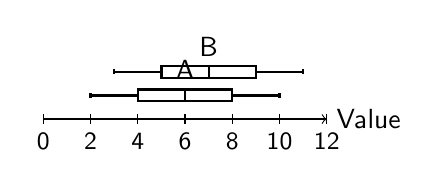
\begin{tikzpicture}[x=0.3cm,y=0.3cm,baseline=(current bounding box.center)]
  % axis
  \draw[->] (0,0) -- (12,0) node[right] {Value};
  \foreach \x in {0,2,4,6,8,10,12} \draw (\x,0.2) -- (\x,-0.2) node[below] {\small \x};
  % boxplot A at y=1
  \draw[thick] (2,1) -- (4,1);
  \draw[thick] (4,0.75) rectangle (8,1.25);
  \draw[thick] (6,0.75) -- (6,1.25);
  \draw[thick] (8,1) -- (10,1);
  \draw[thick] (2,0.9) -- (2,1.1);
  \draw[thick] (10,0.9) -- (10,1.1);
  \node[above] at (6,1.25) {A};
  % boxplot B at y=2
  \draw[thick] (3,2) -- (5,2);
  \draw[thick] (5,1.75) rectangle (9,2.25);
  \draw[thick] (7,1.75) -- (7,2.25);
  \draw[thick] (9,2) -- (11,2);
  \draw[thick] (3,1.9) -- (3,2.1);
  \draw[thick] (11,1.9) -- (11,2.1);
  \node[above] at (7,2.25) {B};
\end{tikzpicture}}
\task {Compare the two box-and-whisker graphs using CSSI.\\[0.4em]
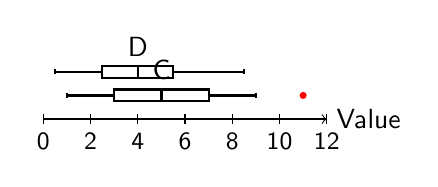
\begin{tikzpicture}[x=0.3cm,y=0.3cm,baseline=(current bounding box.center)]
  \draw[->] (0,0) -- (12,0) node[right] {Value};
  \foreach \x in {0,2,4,6,8,10,12} \draw (\x,0.2) -- (\x,-0.2) node[below] {\small \x};
  % boxplot C with outlier
  \draw[thick] (1,1) -- (3,1);
  \draw[thick] (3,0.75) rectangle (7,1.25);
  \draw[thick] (5,0.75) -- (5,1.25);
  \draw[thick] (7,1) -- (9,1);
  \draw[thick] (1,0.9) -- (1,1.1);
  \draw[thick] (9,0.9) -- (9,1.1);
  \fill[red] (11,1) circle (0.15);
  \node[above] at (5,1.25) {C};
  % boxplot D with skew
  \draw[thick] (0.5,2) -- (2.5,2);
  \draw[thick] (2.5,1.75) rectangle (5.5,2.25);
  \draw[thick] (4,1.75) -- (4,2.25);
  \draw[thick] (5.5,2) -- (8.5,2);
  \draw[thick] (0.5,1.9) -- (0.5,2.1);
  \draw[thick] (8.5,1.9) -- (8.5,2.1);
  \node[above] at (4,2.25) {D};
\end{tikzpicture}}
\task {Compare the two box-and-whisker graphs using CSSI.\\[0.4em]
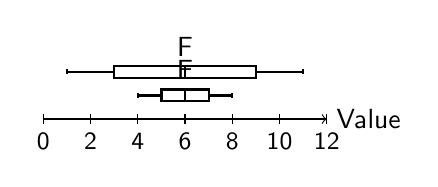
\begin{tikzpicture}[x=0.3cm,y=0.3cm,baseline=(current bounding box.center)]
  \draw[->] (0,0) -- (12,0) node[right] {Value};
  \foreach \x in {0,2,4,6,8,10,12} \draw (\x,0.2) -- (\x,-0.2) node[below] {\small \x};
  % boxplot E tight spread
  \draw[thick] (4,1) -- (5,1);
  \draw[thick] (5,0.75) rectangle (7,1.25);
  \draw[thick] (6,0.75) -- (6,1.25);
  \draw[thick] (7,1) -- (8,1);
  \draw[thick] (4,0.9) -- (4,1.1);
  \draw[thick] (8,0.9) -- (8,1.1);
  \node[above] at (6,1.25) {E};
  % boxplot F wide spread
  \draw[thick] (1,2) -- (3,2);
  \draw[thick] (3,1.75) rectangle (9,2.25);
  \draw[thick] (6,1.75) -- (6,2.25);
  \draw[thick] (9,2) -- (11,2);
  \draw[thick] (1,1.9) -- (1,2.1);
  \draw[thick] (11,1.9) -- (11,2.1);
  \node[above] at (6,2.25) {F};
\end{tikzpicture}}
\task {For each pair of boxplots, compare the centres.}
\task {For each pair of boxplots, compare the shapes.}
\task {For each pair of boxplots, compare the spreads.}
\task {For each pair of boxplots, compare any interesting features.}
\task {Which pair shows the greatest difference in centre? Explain.}
\task {Which pair shows the greatest difference in spread? Explain.}
\task {Which pair shows a clear outlier? Describe its effect on the comparison.}
\task {Which pair shows a skewed distribution? Describe the skewness.}
\task {Explain how you can tell from a boxplot whether the distribution is symmetric or skewed.}
\task {Explain the difference between IQR and range in the context of boxplots.}
\task {Explain how outliers are determined in a boxplot.}
\end{tasks}

\end{document}